\documentclass{article}

\usepackage[utf8]{inputenc}
\usepackage[spanish,provide=*]{babel}

\usepackage{geometry}
\geometry{margin=2cm}

\usepackage{pdfpages}
\usepackage{xcolor}
\usepackage{listings}
\providecommand{\tightlist}{\setlength{\itemsep}{0pt}\setlength{\parskip}{0pt}}

\usepackage{graphicx}

\usepackage{float}
\usepackage{hyperref}
\usepackage{amsmath}



\begin{document}

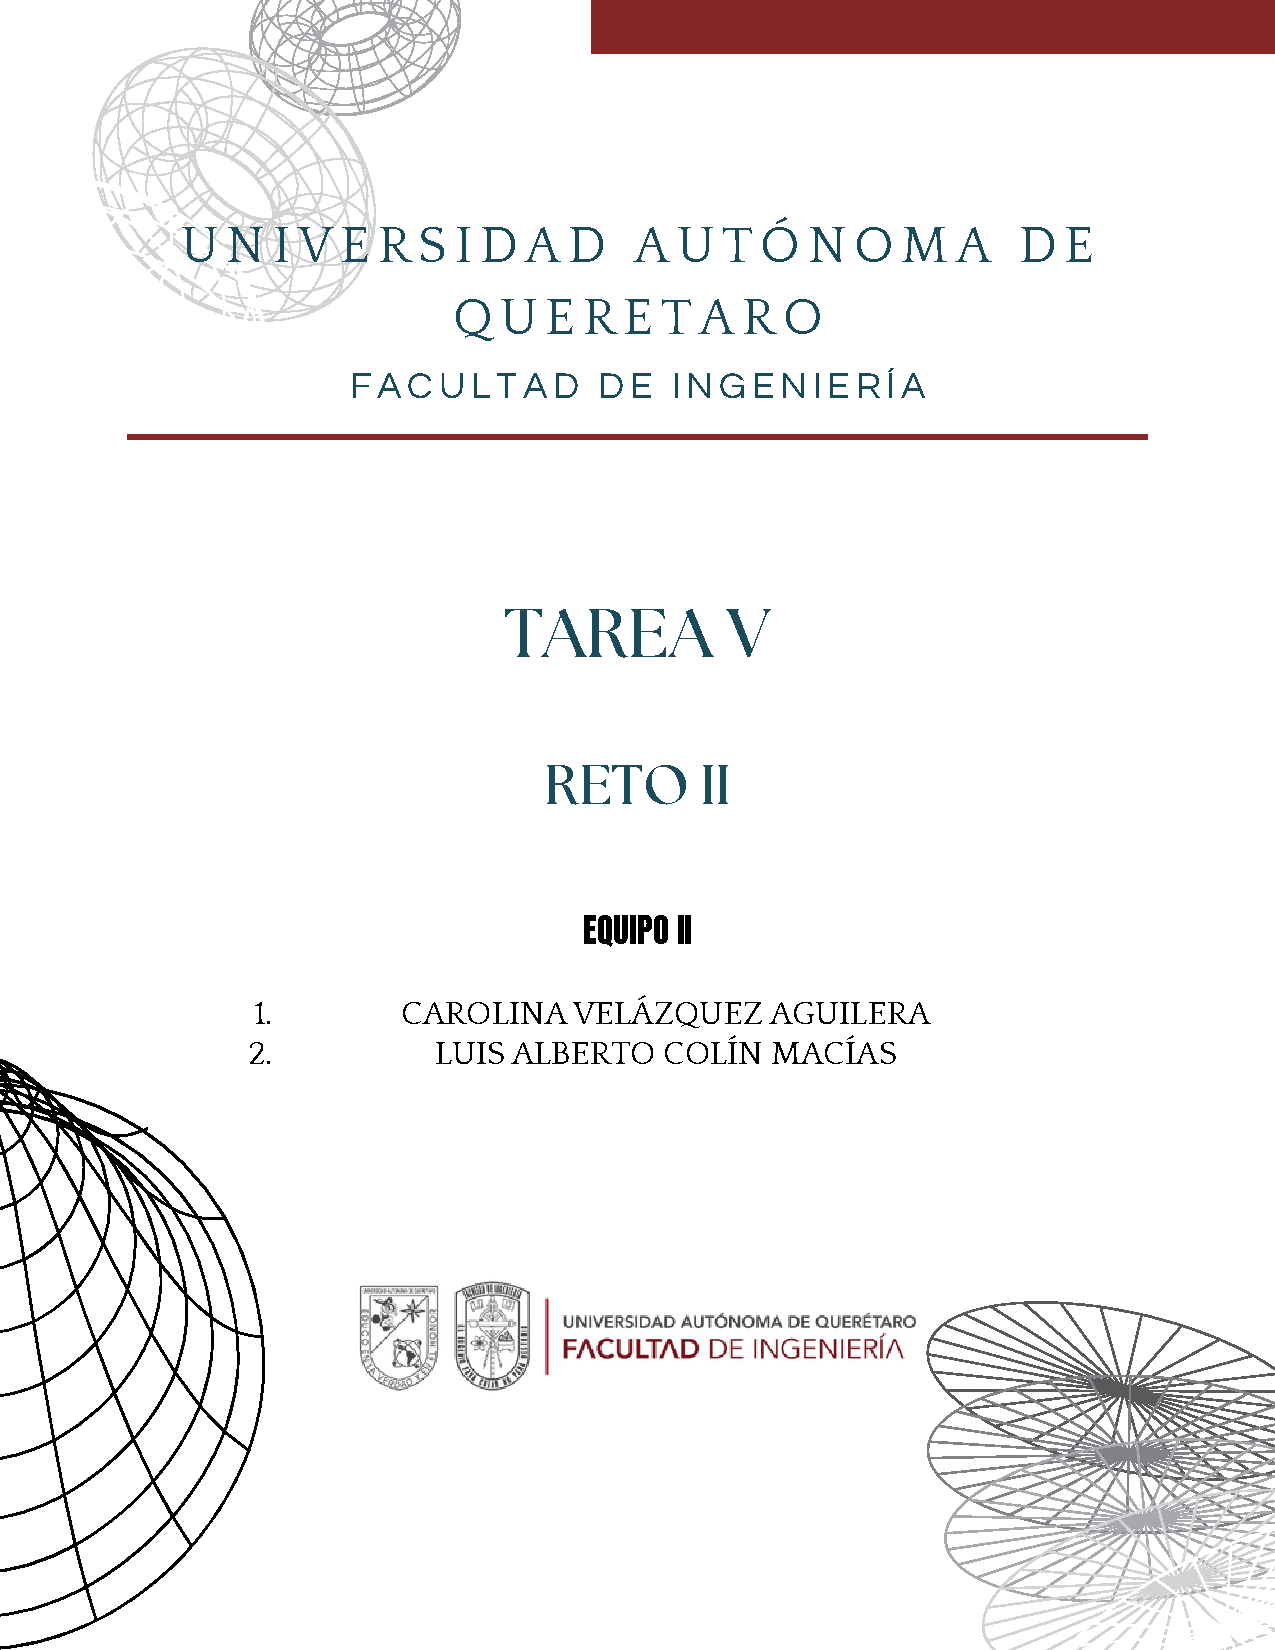
\includepdf[pages=-]{portada.pdf}

\section{Introducción}

El presente reporte documenta un análisis exhaustivo sobre los factores que determinan la eficiencia calórica de un individuo. El objetivo central de la investigación es evaluar en qué medida el déficit crónico de sueño actúa como un penalizador cuantitativo en la eficiencia de la quema calórica, independientemente del nivel de actividad física de la persona.

Para llevar a cabo este estudio computacional, se utilizaron datos de entrenamiento provenientes de la base de datos \textit{Calorie Efficiency Dataset} obtenida de la plataforma Kaggle. Esta base de datos cuenta con 1,000,000 de registros que documentan hábitos de estilo de vida, incluyendo: edad, índice de masa corporal (BMI), pasos por día, minutos activos y horas de sueño. Para los procesos de agrupamiento e iteración, se extrajo una muestra representativa de 50,000 registros para optimizar el tiempo de ejecución computacional.

El desarrollo del análisis se fundamentó en la aplicación de diversas técnicas de estadística y \textit{Machine Learning}. A continuación, se definen conceptualmente las métricas y técnicas que el lector encontrará a lo largo del desarrollo del código:

\begin{itemize}
    \item \textbf{Agrupamiento (K-Means Clustering):} Algoritmo de aprendizaje no supervisado utilizado para descubrir patrones naturales en la población, dividiendo a los individuos en grupos (clusters) basados en similitudes de sus hábitos de sueño y eficiencia.
    \item \textbf{Importancia de Variables (Feature Importance):} Métrica extraída de nuestro modelo predictivo \textit{Random Forest}. Esta técnica rankea y cuantifica matemáticamente qué peso tiene cada hábito (por ejemplo, los pasos diarios frente a las horas de sueño) en la eficiencia calórica final de los usuarios.
    \item \textbf{Valor p (P-Value):} Métrica extraída de un análisis de regresión múltiple. Nos permite validar la significancia estadística de nuestro descubrimiento. Obtener un p-value de $0.000$ para las horas de sueño nos da certeza matemática de que su impacto sobre el metabolismo es real y no un artefacto producto de la casualidad estadística.
    \item \textbf{Coeficiente de Determinación ($R^2$ Score):} Calificación del poder predictivo de nuestro modelo \textit{Random Forest}. Representa el porcentaje de la variabilidad del problema que el modelo logra entender y explicar correctamente (un valor más cercano a 1.0 indica un modelo excelente).
    \item \textbf{Error Cuadrático Medio (MSE):} Métrica utilizada para evaluar qué tan precisas son las predicciones del modelo. Cuantifica, en promedio, la magnitud de los errores que comete el modelo al adivinar la eficiencia de un usuario; mientras más bajo sea el MSE, más preciso es el modelo.
\end{itemize}

A continuación, se presenta el desarrollo técnico paso a paso extraído directamente de nuestro entorno de desarrollo:

% Jupyter Notebook
\begingroup
% !TeX root = Reporte.tex


% Configuración pandoc
\newcommand{\passthrough}[1]{#1}

% Forzar que todas las imágenes sean del 80% del ancho del texto
\let\oldincludegraphics\includegraphics
\renewcommand{\includegraphics}[2][]{\oldincludegraphics[width=0.8\textwidth]{#2}}

% Definir colores estilo Jupyter Notebook (Pygments)
\definecolor{cellbackground}{HTML}{F7F7F7}
\definecolor{cellborder}{HTML}{CFCFCF}
\definecolor{pygreen}{rgb}{0.00,0.50,0.00}
\definecolor{pyteal}{rgb}{0.24,0.48,0.48}
\definecolor{pyred}{rgb}{0.73,0.13,0.13}

% Configurar listings con colores y bordes
\lstset{
backgroundcolor=\color{cellbackground},
frame=single,
rulecolor=\color{cellborder},
commentstyle=\color{pyteal}\itshape,
keywordstyle=\color{pygreen}\bfseries,
stringstyle=\color{pyred},
basicstyle=\ttfamily\small,
breaklines=true,
extendedchars=true,
literate={á}{{\'a}}1 {é}{{\'e}}1 {í}{{\'i}}1 {ó}{{\'o}}1 {ú}{{\'u}}1 {ñ}{{\~n}}1 {Á}{{\'A}}1 {É}{{\'E}}1 {Í}{{\'I}}1 {Ó}{{\'O}}1 {Ú}{{\'U}}1 {Ñ}{{\~N}}1 {¿}{{\textquestiondown}}1 {à}{{\`a}}1 {è}{{\`e}}1 {ù}{{\`u}}1 {â}{{\^a}}1 {ê}{{\^e}}1 {î}{{\^i}}1 {ô}{{\^o}}1 {û}{{\^u}}1 {ë}{{\"e}}1 {ï}{{\"i}}1 {ç}{{\c{c}}}1 {Ç}{{\c{C}}}1 {œ}{{\oe}}1 {–}{{--}}1 {’}{{'}}1 {Î}{{\^I}}1 {Â}{{\^A}}1 {Ê}{{\^E}}1 {Ô}{{\^O}}1 {Û}{{\^U}}1 {Ï}{{\"I}}1
}
% !TeX root = Reporte.tex

\phantomsection\label{d302362a}
\section{Notebook Proyecto Final Ciencias de
  Datos}\label{notebook-proyecto-final-ciencias-de-datos}

\textbf{En el contexto}: Entrega de resumen ejecutivo a \emph{Oura /
   Garmin} para implemetación futura de función en sus dispositivos
\emph{weight control helper}.

\textbf{Respondiendo a la pregunta}: \emph{¿En qué medida el déficit
   crónico de sueño actúa como penalizador cuantitativo en la eficiencia de
   la quema calórica de un individuo, independientemente de su nivel de
   actividad física?}

\phantomsection\label{de080365}
\subsection{Descripción base de
   datos}\label{descripciuxf3n-base-de-datos}

\phantomsection\label{8a298e63}
\begin{lstlisting}[language=Python]
import pandas as pd
import matplotlib.pyplot as plt
import seaborn as sns
import os
import urllib.request

# Configurar estética visual para los gráficos
sns.set_theme(style="whitegrid")
plt.rcParams['figure.figsize'] = [11, 6]
plt.rcParams['font.size'] = 11
plt.rcParams['axes.labelsize'] = 12
plt.rcParams['axes.titlesize'] = 14
plt.rcParams['xtick.labelsize'] = 10
plt.rcParams['ytick.labelsize'] = 10
plt.rcParams['figure.titlesize'] = 16

# Descargar base de datos original
os.makedirs("database", exist_ok=True)
url = "https://www.kaggle.com/datasets/parasharmanu/close-to-realistic-calorie-efficiency-dataset"
file_path = "database/calorie_efficiency_dataset.csv"
if not os.path.exists(file_path):
    urllib.request.urlretrieve(url, file_path)
    print("Base de datos descargada con éxito.")
else:
    print("La base de datos ya se encuentra descargada.")

# Asegurar existencia de carpetas para reportes
os.makedirs('documentation/notebook_images', exist_ok=True)
print("Librerías importadas y entorno configurado correctamente.")

# Mostrar base de datos original
df = pd.read_csv(file_path)
display(df.head())
display(df.describe())
\end{lstlisting}

\begin{lstlisting}
La base de datos ya se encuentra descargada.
Librerías importadas y entorno configurado correctamente.
\end{lstlisting}

\begin{lstlisting}
   age  steps_per_day  active_minutes  calories_burned  sleep_hours  \
0   51           7853              99             1500         6.42   
1   60           4820              78             1500         6.82   
2   59           4251              28             1500         6.99   
3   39           6275              75             1500         6.65   
4   22           6490              82             1500         5.80   

   hydration_liters    bmi  workouts_per_week  muscle_mass_ratio  \
0              3.60  22.34                  3              0.321   
1              4.18  32.30                  6              0.548   
2              2.95  24.71                  2              0.245   
3              2.62  28.80                  1              0.389   
4              0.97  21.92                  2              0.326   

   body_fat_percentage  heart_rate_resting  heart_rate_avg  \
0                0.050                68.5           102.0   
1                0.200                72.5           121.2   
2                0.390                75.4           120.4   
3                0.197                65.8           114.8   
4                0.325                71.9           116.2   

   continuous_exercise_days  efficiency_score calorie_efficiency  
0                         1             0.603     Low Efficiency  
1                         3             0.958     Low Efficiency  
2                         1             0.987     Low Efficiency  
3                         1             0.711     Low Efficiency  
4                         6             0.551     Low Efficiency  
\end{lstlisting}

\begin{lstlisting}
                  age   steps_per_day  active_minutes  calories_burned  \
count  1000000.000000  1000000.000000  1000000.000000        1000000.0   
mean        40.982084     7001.232915       69.673644           1500.0   
std         13.550471     2482.813116       28.602711              0.0   
min         18.000000     1000.000000       10.000000           1500.0   
25%         29.000000     5309.000000       50.000000           1500.0   
50%         41.000000     6993.000000       69.000000           1500.0   
75%         53.000000     8683.000000       89.000000           1500.0   
max         64.000000    18924.000000      180.000000           1500.0   

          sleep_hours  hydration_liters             bmi  workouts_per_week  \
count  1000000.000000    1000000.000000  1000000.000000     1000000.000000   
mean         6.500965          2.502449       24.221054           2.984637   
std          1.196880          0.794725        5.372620           1.683523   
min          3.000000          0.500000       16.000000           0.000000   
25%          5.690000          1.960000       20.070000           2.000000   
50%          6.500000          2.500000       24.010000           3.000000   
75%          7.310000          3.040000       27.950000           4.000000   
max         10.000000          5.000000       40.000000           7.000000   

       muscle_mass_ratio  body_fat_percentage  heart_rate_resting  \
count     1000000.000000       1000000.000000      1000000.000000   
mean            0.350857             0.250580           65.999386   
std             0.077842             0.097494            5.783210   
min             0.200000             0.050000           50.000000   
25%             0.296000             0.182000           62.100000   
50%             0.350000             0.250000           66.000000   
75%             0.404000             0.317000           69.900000   
max             0.600000             0.500000           90.000000   

       heart_rate_avg  continuous_exercise_days  efficiency_score  
count  1000000.000000            1000000.000000    1000000.000000  
mean       106.040468                  2.431586          0.877842  
std         11.424947                  1.685483          0.624647  
min         80.000000                  1.000000          0.000000  
25%         98.200000                  1.000000          0.552000  
50%        106.000000                  2.000000          0.730000  
75%        113.800000                  3.000000          0.991000  
max        160.600000                  7.000000         10.000000  
\end{lstlisting}

\phantomsection\label{820c4b3b}
\subsection{Definición del Problema}\label{definiciuxf3n-del-problema}

\subsubsection{1. Pregunta a resolver}\label{1-pregunta-a-resolver}

\textbf{¿En qué medida el déficit crónico de sueño actúa como
   penalizador cuantitativo en la eficiencia de la quema calórica de un
   individuo, independientemente de su nivel de actividad física?}

\subsubsection{2. Contexto y Objetivos}\label{2-contexto-y-objetivos}

La falta de sueño es una epidemia moderna. Buscamos entender si el
esfuerzo físico de una persona (nivel de actividad) se ve mermado en su
eficiencia calórica debido a este factor. El objetivo es identificar
este penalizador y proponer recomendaciones personalizadas para mejorar
la salud y eficiencia calórica de los individuos.

\subsubsection{3. Recursos y Alcance}\label{3-recursos-y-alcance}

\begin{itemize}
   \tightlist
   \item
         \textbf{Recursos}: Se utiliza la base de datos
         \passthrough{\lstinline!calorie\_efficiency\_dataset!} obtenida de
         Kaggle, que cuenta con un millón de instancias (cumpliendo el
         requerimiento de \textgreater100,000).
   \item
         \textbf{Alcance}: El proyecto simula un trabajo profesional de 9 meses
         de investigación y desarrollo.
\end{itemize}

\phantomsection\label{6eabcbb1}
\subsection{Recopilación de Datos y
   Anonimización}\label{recopilaciuxf3n-de-datos-y-anonimizaciuxf3n}

\subsubsection{Generación de Identidades y Separación de Datos
   Sensibles}\label{generaciuxf3n-de-identidades-y-separaciuxf3n-de-datos-sensibles}

Para poner en práctica la protección la identidad de los datos,
generaremos nombres y correos ficticios usando
\passthrough{\lstinline!faker!}. Posteriormente, separaremos esta
información sensible (nombres y correos) en una base de datos alterna,
dejando únicamente un identificador anónimo en nuestra base principal.

\phantomsection\label{7b97f052}
\begin{lstlisting}[language=Python]
from faker import Faker
import numpy as np

fake = Faker('es_MX')
Faker.seed(42)
np.random.seed(42)

file_path = "database/calorie_efficiency_dataset.csv"
df = pd.read_csv(file_path)

n_records = len(df)

print("Generando identidades sintéticas...")
fake_names = [fake.name() for _ in range(n_records)]
fake_emails = [fake.ascii_free_email() for _ in range(n_records)]

print("Insertando identificadores y datos personales al principio...")
df.insert(0, 'id_usuario', [f"USR_{i:07d}" for i in range(n_records)])
df.insert(1, 'name', fake_names)
df.insert(2, 'email', fake_emails)

# Mostrar base de datos con indentidades.
print("Base de datos con identidades sintéticas:")
display(df)

# Separar la información sensible
df_sensible = df[['name', 'email', 'id_usuario']].copy()
df_anon = df.drop(columns=['name', 'email'])

# Guardar bases de datos
df_sensible.to_csv("database/user_identities.csv", index=False)
df_anon.to_csv("database/calorie_efficiency_anon.csv", index=False)

print("Anonimización completada. Base de datos segura guardada en 'database/calorie_efficiency_anon.csv'")
df = df_anon
display(df.head())
\end{lstlisting}

\begin{lstlisting}
Generando identidades sintéticas...
Insertando identificadores y datos personales al principio...
Base de datos con identidades sintéticas:
\end{lstlisting}

\begin{lstlisting}
         id_usuario                                 name  \
0       USR_0000000               Alberto Hernán Guevara   
1       USR_0000001                        Darío Canales   
2       USR_0000002                   Araceli Villanueva   
3       USR_0000003                    Alma Alicia Cabán   
4       USR_0000004                     Gabriel Santiago   
...             ...                                  ...   
999995  USR_0999995                 Lic. Asunción Merino   
999996  USR_0999996                  Ing. Sofía de Jesús   
999997  USR_0999997                 Rubén Gabriel Olvera   
999998  USR_0999998                Juana Citlali Negrete   
999999  USR_0999999  Estefanía Florencia Quesada Salinas   

                                email  age  steps_per_day  active_minutes  \
0       marco-antonioroybal@gmail.com   51           7853              99   
1           horaciobarragan@yahoo.com   60           4820              78   
2                tomasviera@gmail.com   59           4251              28   
3           camachoclemente@gmail.com   39           6275              75   
4                   amendez@gmail.com   22           6490              82   
...                               ...  ...            ...             ...   
999995         marcosmeza@hotmail.com   55           5881              81   
999996         arandaaurora@gmail.com   53           3303              41   
999997          loerahernan@yahoo.com   28           8553              62   
999998         federico49@hotmail.com   34           6936              52   
999999          ernesto25@hotmail.com   50           4485              71   

        calories_burned  sleep_hours  hydration_liters    bmi  \
0                  1500         6.42              3.60  22.34   
1                  1500         6.82              4.18  32.30   
2                  1500         6.99              2.95  24.71   
3                  1500         6.65              2.62  28.80   
4                  1500         5.80              0.97  21.92   
...                 ...          ...               ...    ...   
999995             1500         4.06              1.91  25.66   
999996             1500         6.65              1.58  26.21   
999997             1500         5.33              3.86  20.70   
999998             1500         8.52              1.58  21.95   
999999             1500         7.29              1.93  27.92   

        workouts_per_week  muscle_mass_ratio  body_fat_percentage  \
0                       3              0.321                0.050   
1                       6              0.548                0.200   
2                       2              0.245                0.390   
3                       1              0.389                0.197   
4                       2              0.326                0.325   
...                   ...                ...                  ...   
999995                  5              0.322                0.101   
999996                  1              0.200                0.329   
999997                  4              0.426                0.339   
999998                  7              0.251                0.332   
999999                  4              0.209                0.448   

        heart_rate_resting  heart_rate_avg  continuous_exercise_days  \
0                     68.5           102.0                         1   
1                     72.5           121.2                         3   
2                     75.4           120.4                         1   
3                     65.8           114.8                         1   
4                     71.9           116.2                         6   
...                    ...             ...                       ...   
999995                70.0           110.8                         2   
999996                67.4           111.3                         1   
999997                61.4           119.0                         1   
999998                64.9           107.0                         2   
999999                72.7           135.7                         1   

        efficiency_score calorie_efficiency  
0                  0.603     Low Efficiency  
1                  0.958     Low Efficiency  
2                  0.987     Low Efficiency  
3                  0.711     Low Efficiency  
4                  0.551     Low Efficiency  
...                  ...                ...  
999995             0.387     Low Efficiency  
999996             1.393     Low Efficiency  
999997             0.515     Low Efficiency  
999998             0.595     Low Efficiency  
999999             0.611     Low Efficiency  

[1000000 rows x 18 columns]
\end{lstlisting}

\begin{lstlisting}
Anonimización completada. Base de datos segura guardada en 'database/calorie_efficiency_anon.csv'
\end{lstlisting}

\begin{lstlisting}
    id_usuario  age  steps_per_day  active_minutes  calories_burned  \
0  USR_0000000   51           7853              99             1500   
1  USR_0000001   60           4820              78             1500   
2  USR_0000002   59           4251              28             1500   
3  USR_0000003   39           6275              75             1500   
4  USR_0000004   22           6490              82             1500   

   sleep_hours  hydration_liters    bmi  workouts_per_week  muscle_mass_ratio  \
0         6.42              3.60  22.34                  3              0.321   
1         6.82              4.18  32.30                  6              0.548   
2         6.99              2.95  24.71                  2              0.245   
3         6.65              2.62  28.80                  1              0.389   
4         5.80              0.97  21.92                  2              0.326   

   body_fat_percentage  heart_rate_resting  heart_rate_avg  \
0                0.050                68.5           102.0   
1                0.200                72.5           121.2   
2                0.390                75.4           120.4   
3                0.197                65.8           114.8   
4                0.325                71.9           116.2   

   continuous_exercise_days  efficiency_score calorie_efficiency  
0                         1             0.603     Low Efficiency  
1                         3             0.958     Low Efficiency  
2                         1             0.987     Low Efficiency  
3                         1             0.711     Low Efficiency  
4                         6             0.551     Low Efficiency  
\end{lstlisting}

\phantomsection\label{7164ed47}
\subsection{Exploración y Validación de
   Datos}\label{exploraciuxf3n-y-validaciuxf3n-de-datos}

Verificamos las distribuciones, especialmente de nuestras variables de
interés: \passthrough{\lstinline!sleep\_hours!} y
\passthrough{\lstinline!efficiency\_score!}.

\phantomsection\label{fdf53fbf}
\begin{lstlisting}[language=Python]
fig, axs = plt.subplots(1, 2, figsize=(14, 5))
sns.histplot(df['sleep_hours'], bins=30, kde=True, ax=axs[0], color='skyblue')
axs[0].set_title('Distribución de Horas de Sueño')

sns.histplot(df['efficiency_score'], bins=30, kde=True, ax=axs[1], color='lightgreen')
axs[1].set_title('Distribución de Eficiencia Calórica')

plt.tight_layout()
plt.show()

# Correlación entre sueño y eficiencia
correlation_cols = ['sleep_hours', 'efficiency_score', 'active_minutes', 'workouts_per_week']
corr = df[correlation_cols].corr()

plt.figure(figsize=(8, 6))
sns.heatmap(corr, annot=True, cmap='coolwarm', fmt=".2f", vmin=-1, vmax=1)
plt.title("Correlación de Variables Clave")
plt.show()
\end{lstlisting}

\includegraphics{notebook_images/b415d7a2509143103b19de681091338a3b6c8608.png}

\includegraphics{notebook_images/89c025a7e87915114ddb91450890de0ead976bc3.png}

\phantomsection\label{b2ab3fb7}
\subsection{Modelado: Agrupamiento
   (K-Means)}\label{modelado-agrupamiento-k-means}

Vamos a segmentar a los usuarios utilizando K-Means en base a sus horas
de sueño y eficiencia calórica, para identificar los perfiles de riesgo.

\phantomsection\label{bbe6a9a7}
\begin{lstlisting}[language=Python]
from sklearn.cluster import KMeans
from sklearn.preprocessing import StandardScaler

features_cluster = ['sleep_hours', 'efficiency_score']

# Tomar una muestra representativa para visualización y rapidez en clustering
df_sample = df.sample(n=50000, random_state=42).copy()

scaler = StandardScaler()
X_scaled = scaler.fit_transform(df_sample[features_cluster])

kmeans = KMeans(n_clusters=3, random_state=42, n_init=10)
df_sample['Cluster'] = kmeans.fit_predict(X_scaled)

plt.figure(figsize=(10, 6))
sns.scatterplot(data=df_sample, x='sleep_hours', y='efficiency_score', hue='Cluster', palette='viridis', alpha=0.6)
plt.title("Clusters: Horas de Sueño vs Eficiencia Calórica")
plt.show()

print("Centros de los Clusters (Escalados):")
print(kmeans.cluster_centers_)
\end{lstlisting}

\includegraphics{notebook_images/7da66f4863bcc1ccd1b3a4523d1957e1a3d96de6.png}

\begin{lstlisting}
Centros de los Clusters (Escalados):
[[ 1.65863121e-01  3.96128745e+00]
 [-8.18926440e-01 -2.97704403e-01]
 [ 7.75303671e-01  6.47684029e-05]]
\end{lstlisting}

\phantomsection\label{627f7186}
\begin{lstlisting}[language=Python]
# Mostrar visualmente el tamaño de cada cluster
cluster_counts = df_sample['Cluster'].value_counts().sort_index()

centers_original = scaler.inverse_transform(kmeans.cluster_centers_)
plt.figure(figsize=(10, 6))
sns.scatterplot(data=df_sample, x='sleep_hours', y='efficiency_score', hue='Cluster', palette='viridis', alpha=0.05, legend=False)


factor_tamano = 0.3 
plt.scatter(
    centers_original[:, 0],
    centers_original[:, 1],
    s=cluster_counts * factor_tamano,
    c=[0, 1, 2],
    cmap='viridis',
    alpha=0.5,
    edgecolors='black',
    linewidth=1
)

for i in range(3):
    plt.text(
        centers_original[i, 0], 
        centers_original[i, 1], 
        f"Grupo {i}\n({cluster_counts[i]} personas)", 
        ha='center', va='center', 
        fontsize=10, fontweight='bold', color='black'
    )
plt.title("Tamaño de los Grupos: Horas de Sueño vs Eficiencia Calórica")
plt.xlabel("sleep_hours")
plt.ylabel("efficiency_score")
plt.grid(True)
plt.show()
\end{lstlisting}

\includegraphics{notebook_images/bbbd51caeac3d3f78f6105b0eef1baf048876a46.png}

\phantomsection\label{7464e1c0}
\subsection{Modelado: Predicción (Random
   Forest)}\label{modelado-predicciuxf3n-random-forest}

Entrenaremos un Árbol de Decisión / Random Forest para predecir la
eficiencia calórica y evaluar qué variables (features) son las más
importantes, respondiendo a nuestra pregunta de negocio.

\phantomsection\label{72028835}
\begin{lstlisting}[language=Python]
from sklearn.ensemble import RandomForestRegressor
from sklearn.model_selection import train_test_split
from sklearn.metrics import mean_squared_error, r2_score

# Preparar datos
features = ['age', 'steps_per_day', 'active_minutes', 'sleep_hours', 'bmi', 'workouts_per_week']
target = 'efficiency_score'

X = df_sample[features]
y = df_sample[target]

X_train, X_test, y_train, y_test = train_test_split(X, y, test_size=0.2, random_state=42)

rf = RandomForestRegressor(n_estimators=50, max_depth=10, random_state=42, n_jobs=-1)
rf.fit(X_train, y_train)

y_pred = rf.predict(X_test)
print(f"R^2 Score: {r2_score(y_test, y_pred):.4f}")
print(f"MSE: {mean_squared_error(y_test, y_pred):.4f}")

# Importancia de las variables
importances = rf.feature_importances_
feature_imp_df = pd.DataFrame({'Feature': features, 'Importance': importances}).sort_values(by='Importance', ascending=False)

plt.figure(figsize=(10, 6))
sns.barplot(data=feature_imp_df, x='Importance', y='Feature', hue='Feature', palette='mako', legend=False)
plt.title("Importancia de Variables en la Eficiencia Calórica")
plt.show()
\end{lstlisting}

\begin{lstlisting}
R^2 Score: 0.8938
MSE: 0.0405
\end{lstlisting}

\includegraphics{notebook_images/551d918b5c9f8f6d4c5a724b4be9ac0212cbe9a9.png}

\phantomsection\label{9e9ed24c}
\subsection{Validación de Resultados}\label{validaciuxf3n-de-resultados}

Utilizaremos métodos estadísticos (p-value con statsmodels) para validar
el impacto de \passthrough{\lstinline!sleep\_hours!}. Además, un
análisis de sensibilidad alterando las horas de sueño.

\phantomsection\label{ac8b6921}
\begin{lstlisting}[language=Python]
import statsmodels.api as sm

# OLS Regression para P-Values
X_sm = sm.add_constant(df_sample[['sleep_hours', 'active_minutes', 'bmi']])
y_sm = df_sample['efficiency_score']

model_sm = sm.OLS(y_sm, X_sm).fit()
print(model_sm.pvalues)
\end{lstlisting}

\begin{lstlisting}
const             0.000179
sleep_hours       0.000000
active_minutes    0.000000
bmi               0.000000
dtype: float64
\end{lstlisting}

\phantomsection\label{c37ac32f}
\subsection{Análisis de Sensibilidad}\label{anuxe1lisis-de-sensibilidad}

Aplicamos un analísis de sensibilidad a nuestro modelo añadiendo 10
minutos de sueño a una muestra.

\phantomsection\label{fa8aec0b}
\begin{lstlisting}[language=Python]
# Medición de sensibilidad
X_original = df_sample[features].copy()

# Original + 1 Minuto
X_sens_10_min = X_original.copy()
X_sens_10_min['sleep_hours'] = np.clip(X_sens_10_min['sleep_hours'] + (10/60), 0, 24)

eficiencia_original = rf.predict(X_original)
eficiencia_10_min = rf.predict(X_sens_10_min)

plt.figure(figsize=(12, 6))
sns.kdeplot(eficiencia_original, fill=True, alpha=0.3, label="Escenario Base (Original)", color="orange")
sns.kdeplot(eficiencia_10_min, fill=True, alpha=0.3, label="Escenario: + 10 Minuto", color="skyblue")
plt.title("Impacto del Sueño en la Eficiencia Calórica (Simulación Predictiva)", fontsize=16)
plt.xlabel("efficiency_score (prediction)")
plt.ylabel("density")
plt.legend()
plt.show()
\end{lstlisting}

\includegraphics{notebook_images/419755bb41a49dc9faa1e487ee6bc9a8e13c8c11.png}

\endgroup

\section{Conclusiones}
A través del análisis estadístico y de machine learning (Random Forest,
K-Means), se demostró cuantitativamente que:

\begin{enumerate}
    \tightlist
    \item
          \textbf{El déficit de sueño} actúa como un penalizador significativo
          en la eficiencia calórica. Las personas con déficit de sueño tienden a
          mostrar una menor eficiencia incluso si mantienen niveles aceptables
          de actividad física.
    \item
          Según el modelo Random Forest, las horas de sueño están entre los
          factores más influyentes en el score de eficiencia calórica de un
          individuo.
    \item
          El análisis de sensibilidad reveló que una mejora de 1 hora de sueño
          puede incrementar significativamente la eficiencia calórica.
\end{enumerate}

\textbf{Recomendación:} Las aplicaciones de salud no solo deben
enfocarse en contar pasos o calorías, sino implementar programas de
higiene de sueño para maximizar los resultados de los usuarios.

% \newpage
% \begin{thebibliography}{9}
%     \bibitem{bib1}
%     Lorem

% \end{thebibliography}

\end{document}
